
\section{Using the previous interpolants to keep the weight parameters at 1}
\label{section:keeping_alpha_at_1}
One idea to solve the problem of the loss in accuracy due to deviation of the $\alpha$ and $\beta$ parameters from 1 is to construct the interpolant using a value of 1 for these parameters. We note that the best accuracy we can hope to get is with a value of 1 and thus employing data values situated at uniform distances apart guarantees the minimum error.

\subsection{rk4 with HB6} For the HB6 case, a simple way to guarantee that the value of $\alpha$ is 1 is by using the previous interpolants to get the required values at $x_{i - 1}=x_i - h$. Say we are at a value $x_i$ and we took a step of size $h$ to get to the value $x_{i + 1}$ where the function evaluation was $f_{i + 1}$ and the solution was $y_{i + 1}$. We could use the previous interpolants defined on the range $[0, x_i]$ to get a value at $x_i - h$ for the solution approximation, $y_{i - 1}$, and then we can use this $y_{i-1}$ value to compute $f(t_{i-1}, y_{i-1})$ to get the derivative $f_{i - 1}$.  We could thus create the new interpolant using these data points to guarantee that $\alpha$ stays at 1. This technique costs one extra function evaluation to obtain $f_{i-1}$.

This technique works (see Figures $\ref{fig:static_alpha_rk4_with_hb6_p1_global_defect}$ to $\ref{fig:static_alpha_rk4_with_hb6_p3_scaled_defects}$ to see the defect being controlled) but will require that the step-size is artificially limited on the first few steps so that we can interpolant back $x_i - h$ and still be in a range where our interpolants are correctly defined. For example, If we go from $t_0$ to $t_0 + h$ and the error estimate is much lower than the tolerance, we cannot use a step size of $2h$ as $t_0 + h - 2h$ = $t_0-h$ because we do not have an interpolant in the region $\leq t_0$. However this is not an issue as we can perform the first few steps with a CRK scheme for example.

\paragraph{Problem 1 results}
Figures $\ref{fig:static_alpha_rk4_with_hb6_p1_global_defect}$, $\ref{fig:static_alpha_rk4_with_hb6_p1_global_error}$ and $\ref{fig:static_alpha_rk4_with_hb6_p1_scaled_defects}$ shows the results of using the RK4 with HB6 and $\alpha = 1$ on Problem 1. We note that an absolute tolerance of $10^{-6}$ is applied on the maximum defect within the step and this can be shown to occur at $0.3h$ and $0.8h$ along a step of size, h. See Figure $\ref{fig:static_alpha_rk4_with_hb6_p1_scaled_defects}$, to see the scaled defect reaching a maximum near these points. We note that we are able to successfully control the defect of the continuous numerical solution using this approach, see Figure $\ref{fig:static_alpha_rk4_with_hb6_p1_global_defect}$. 


\begin{figure}[H]
\centering
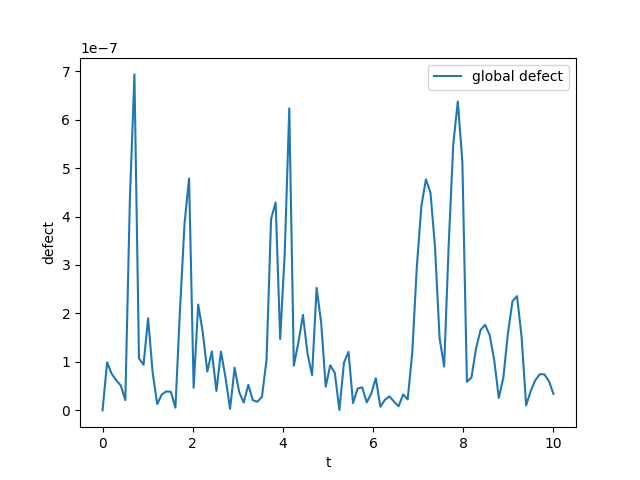
\includegraphics[width=0.7\linewidth]{./figures/static_alpha_rk4_with_hb6_p1_global_defect}
\caption{Defect across the entire domain for RK4 with HB6 using $\alpha$ = 1 on problem 1 at an absolute tolerance of $10^{-6}$.}
\label{fig:static_alpha_rk4_with_hb6_p1_global_defect}
\end{figure}

\begin{figure}[H]
\centering
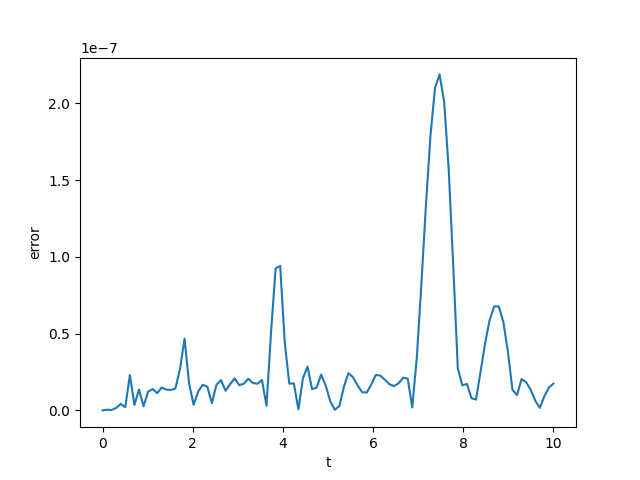
\includegraphics[width=0.7\linewidth]{./figures/static_alpha_rk4_with_hb6_p1_global_error}
\caption{Global Error for RK4 with HB6 using $\alpha$ = 1 on problem 1 at an absolute tolerance of $10^{-6}$.}
\label{fig:static_alpha_rk4_with_hb6_p1_global_error}
\end{figure}

\begin{figure}[H]
\centering
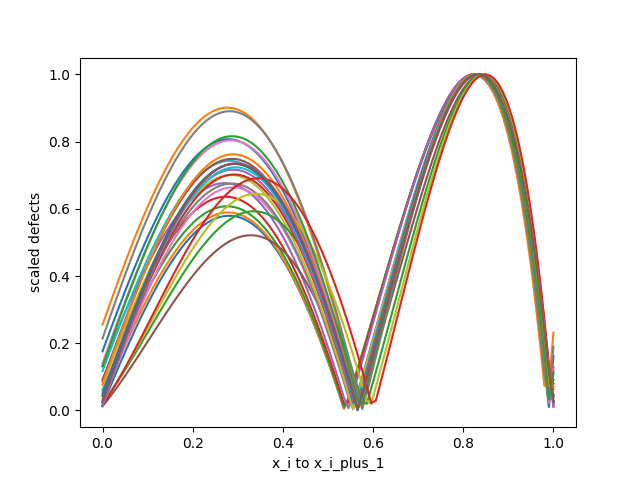
\includegraphics[width=0.7\linewidth]{./figures/static_alpha_rk4_with_hb6_p1_scaled_defects}
\caption{Scaled defects for RK4 with HB6 using $\alpha$ = 1 on problem 1 at an absolute tolerance of $10^{-6}$ mapped onto $[0, 1]$.}
\label{fig:static_alpha_rk4_with_hb6_p1_scaled_defects}
\end{figure}

\paragraph{Problem 2 results}
Figures $\ref{fig:static_alpha_rk4_with_hb6_p2_global_defect}$, $\ref{fig:static_alpha_rk4_with_hb6_p2_global_error}$ and $\ref{fig:static_alpha_rk4_with_hb6_p2_scaled_defects}$ shows the results of using RK4 with HB6 and $\alpha = 1$ on Problem 2. We note that an absolute tolerance of $10^{-6}$ is applied on the maximum defect within the step and this can be shown to occur at $0.8h$ along a step of size, h. See Figure $\ref{fig:static_alpha_rk4_with_hb6_p2_scaled_defects}$, to see the scaled defect reaching a maximum near these points. We note that we are able to successfully control the defect of the continuous numerical solution using this approach, see Figure $\ref{fig:static_alpha_rk4_with_hb6_p2_global_defect}$. 
\begin{figure}[H]
\centering
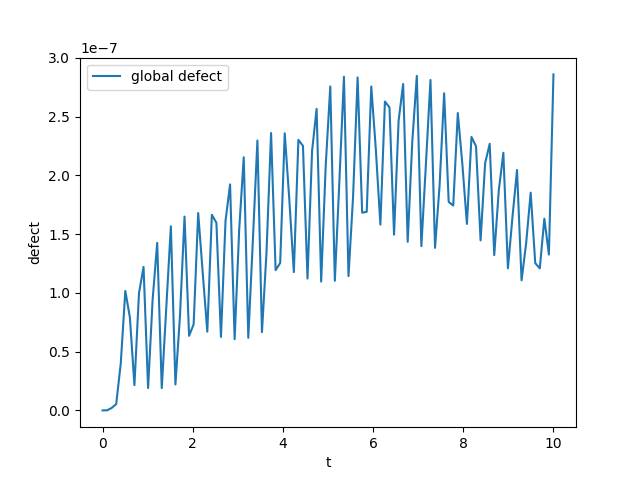
\includegraphics[width=0.7\linewidth]{./figures/static_alpha_rk4_with_hb6_p2_global_defect}
\caption{Defect across the entire domain for RK4 with HB6 using $\alpha$ = 1 on problem 2 at an absolute tolerance of $10^{-6}$.}
\label{fig:static_alpha_rk4_with_hb6_p2_global_defect}
\end{figure}

\begin{figure}[H]
\centering
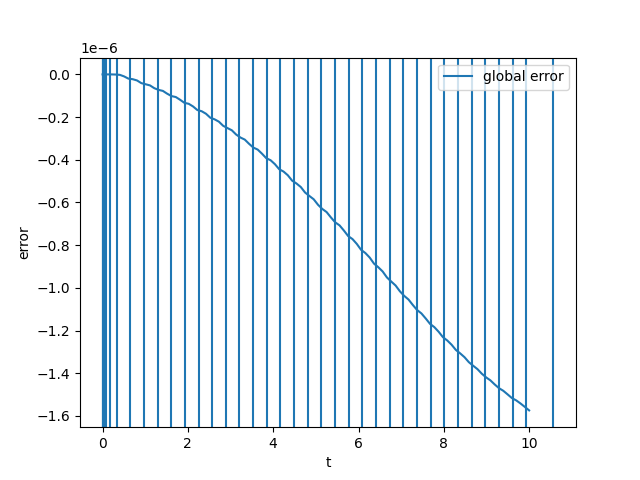
\includegraphics[width=0.7\linewidth]{./figures/static_alpha_rk4_with_hb6_p2_global_error}
\caption{Global Error for RK4 with HB6 using $\alpha$ = 1 on problem 2 at an absolute tolerance of $10^{-6}$.}
\label{fig:static_alpha_rk4_with_hb6_p2_global_error}
\end{figure}

\begin{figure}[H]
\centering
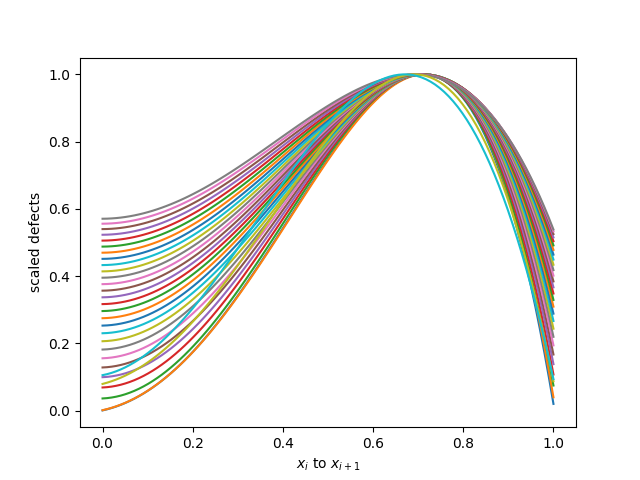
\includegraphics[width=0.7\linewidth]{./figures/static_alpha_rk4_with_hb6_p2_scaled_defects}
\caption{Scaled defects for RK4 with HB6 using $\alpha$ = 1 on problem 2 at an absolute tolerance of $10^{-6}$ mapped onto $[0, 1]$.}
\label{fig:static_alpha_rk4_with_hb6_p2_scaled_defects}
\end{figure}

\begin{figure}[H]
\centering
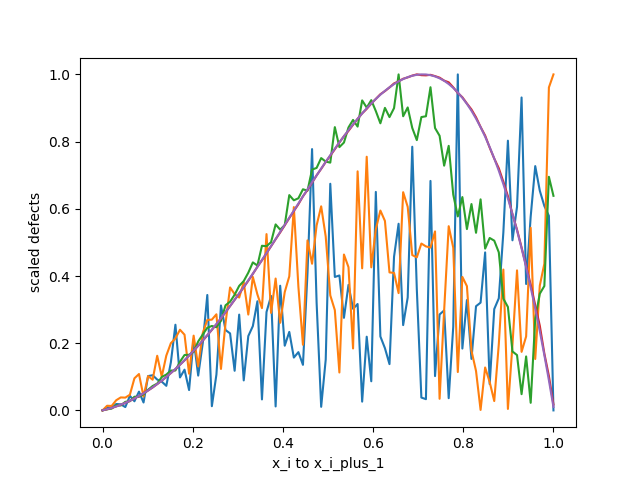
\includegraphics[width=0.7\linewidth]{./figures/static_alpha_rk4_with_hb6_p2_scaled_defects_small_steps}
\caption{Scaled defects for RK4 with HB6 using $\alpha$ = 1 on small steps on problem 2 at an absolute tolerance of $10^{-6}$ mapped onto $[0, 1]$. Despite the noise, the maximum defect mostly appears near $0.8h$.}
\label{fig:static_alpha_rk4_with_hb6_p2_scaled_defects_small_steps}
\end{figure}

\paragraph{Problem 3 results}
Figures $\ref{fig:static_alpha_rk4_with_hb6_p3_global_defect}$, $\ref{fig:static_alpha_rk4_with_hb6_p3_global_error}$ and $\ref{fig:static_alpha_rk4_with_hb6_p3_scaled_defects}$ shows the results of using RK4 with HB6 and $\alpha = 1$ on Problem 3. We note that an absolute tolerance of $10^{-6}$ is applied on the maximum defect within the step and this can be shown to occur at $0.3h$ or $0.8h$along a step of size, h though this problem produces a more diverse location for the peaks. See Figure $\ref{fig:static_alpha_rk4_with_hb6_p3_scaled_defects}$, to see the scaled defect reaching a maximum near these points. We note that we are able to successfully control the defect of the continuous numerical solution using this approach, see Figure $\ref{fig:static_alpha_rk4_with_hb6_p3_global_defect}$. 

\begin{figure}[H]
\centering
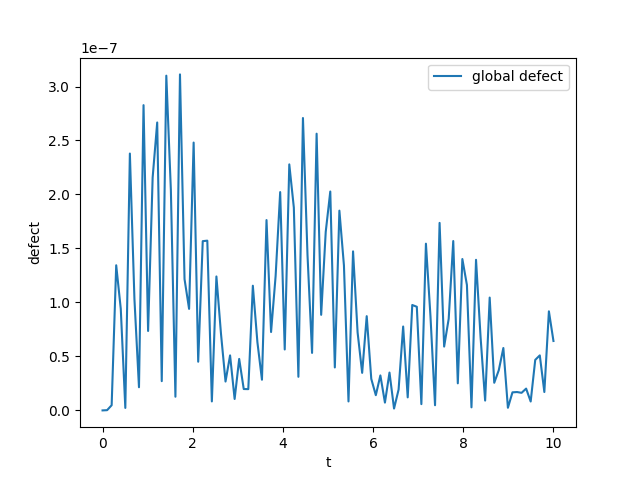
\includegraphics[width=0.7\linewidth]{./figures/static_alpha_rk4_with_hb6_p3_global_defect}
\caption{Defect across the entire domain for RK4 with HB6 using $\alpha$ = 1 on problem 3 at an absolute tolerance of $10^{-6}$.}
\label{fig:static_alpha_rk4_with_hb6_p3_global_defect}
\end{figure}

\begin{figure}[H]
\centering
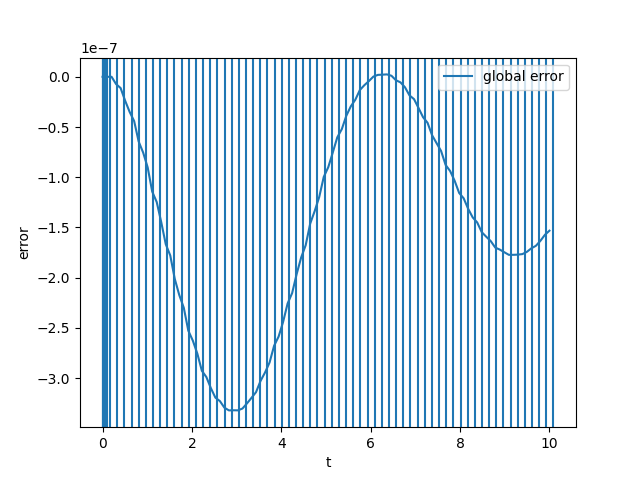
\includegraphics[width=0.7\linewidth]{./figures/static_alpha_rk4_with_hb6_p3_global_error}
\caption{Global Error for RK4 with HB6 using $\alpha$ = 1 on problem 3 at an absolute tolerance of $10^{-6}$.}
\label{fig:static_alpha_rk4_with_hb6_p3_global_error}
\end{figure}

\begin{figure}[H]
\centering
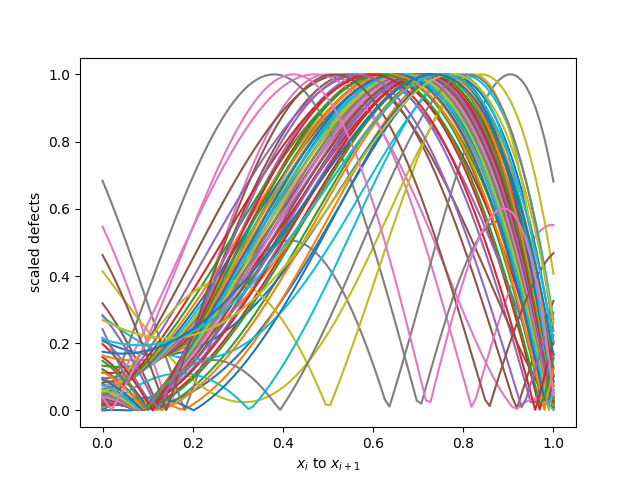
\includegraphics[width=0.7\linewidth]{./figures/static_alpha_rk4_with_hb6_p3_scaled_defects}
\caption{Scaled defects for RK4 with HB6 using $\alpha$ = 1 on problem 3 at an absolute tolerance of $10^{-6}$ mapped onto $[0, 1]$.}
\label{fig:static_alpha_rk4_with_hb6_p3_scaled_defects}
\end{figure}

\begin{table}[h]
\caption {Number of steps taken by RK4 when modified to do defect control with HB6 when we fix $\alpha$ at 1 vs when we allow it to fluctuate during the integration.} \label{tab:rk4_with_hb6_static_vs_variable_alpha}
\begin{center}
\begin{tabular}{ c c c c c } 
Problem & succ. steps & $\alpha$=1 succ. & nsteps & $\alpha$=1 nsteps \\ 
1       & 27                      &        29               & 27         & 33\\ 
2       & 36                      &        34               & 40         & 36\\
3       & 62                      &        65               & 73         & 82\\
\end{tabular}
\end{center}
\end{table}

Table $\ref{tab:rk4_with_hb6_static_vs_variable_alpha}$ shows how the solver with $\alpha$ fixed at 1 and the solver with $\alpha$ allowed to vary differ in the number of steps that they take. The results are very similar because, as we noted before, $\alpha$ tends to stay close to 1 and rarely deviates to a value smaller than $\frac{1}{4}$ or larger than 4.

\subsection{rk6 with HB8} For the HB8 case, a simple way to guarantee that the values of $\alpha$ and $\beta$ are 1 is by using the previous interpolants to get the required values at $x_{i - 1}=x_i-h$ and $x_{i - 2}=x_i-2h$. Suppose that we are at $x_i$ and we took a step of size $h$ to get to the value $x_{i + 1}$ where the function evaluation was $f_{i + 1}$ and the solution was $y_{i + 1}$. We could get the values of the solution and the derivative by using the previous interpolants defined on the range $[0, x_i]$ to get the value at exactly $x_i - h$ for the solution, $y_{i - 1}$, and then evaluate $f(t_{i-1}, y_{i-1})$ to get the derivative $f_{i - 1}$.  We can also use the previous interpolants on $[0, x_i]$ to get the values of the solution, $y_{i-2}$ and use it to evaluate $f(t_{i-2}, y_{i-2})$ to get the values of the derivative, $f_{i-2}$, at $x_{i-2} = x_i - 2h$. We could thus create create the new interpolant using the data values defined as such to guarantee that $\alpha$ and $\beta$ equal to 1. We note that we have built interpolants for both the solution and the derivative that  can interpolate up to $x_i$ for all cases except for the case $x_i = 0$ or for the first few steps. This scheme uses two more function evaluations.

This technique works (see Figures $\ref{fig:static_alpha_rk6_with_hb8_p1_global_defect}$ to $\ref{fig:static_alpha_rk6_with_hb8_p3_scaled_defects_small_steps}$ to see the defect being controlled) but will require that the step-size is artificially limited on the first few steps so that we can interpolant back $x_i - h$ and/or $x_i - 2h$ and still be in a range where our interpolants are correctly defined. This is not an issue as a CRK scheme could be used for the first few steps.

\paragraph{Problem 1 results}
Figures $\ref{fig:static_alpha_rk6_with_hb8_p1_global_defect}$, $\ref{fig:static_alpha_rk6_with_hb8_p1_global_error}$ and $\ref{fig:static_alpha_rk6_with_hb8_p1_scaled_defects}$ shows the results of using RK6 with HB8 and $\alpha = 1$ and $\beta = 1$ on Problem 1. We note that an absolute tolerance of $10^{-6}$ is applied on the maximum defect within the step and this can be shown to occur at $0.4h$ or $0.8h$ along a step of size, h. See Figure $\ref{fig:static_alpha_rk6_with_hb8_p1_scaled_defects}$, to see the scaled defect reaching a maximum near these points. We note that we are able to successfully control the defect of the continuous numerical solution using this approach, see Figure $\ref{fig:static_alpha_rk6_with_hb8_p1_global_defect}$. 
\begin{figure}[H]
\centering
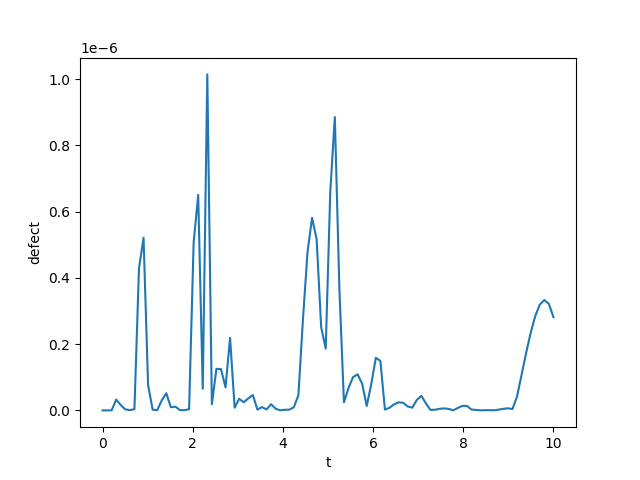
\includegraphics[width=0.7\linewidth]{./figures/static_alpha_rk6_with_hb8_p1_global_defect}
\caption{Defect across the entire domain for RK6 with HB8 using $\alpha$ and $\beta$ = 1 on problem 1 at an absolute tolerance of $10^{-6}$.}
\label{fig:static_alpha_rk6_with_hb8_p1_global_defect}
\end{figure}

\begin{figure}[H]
\centering
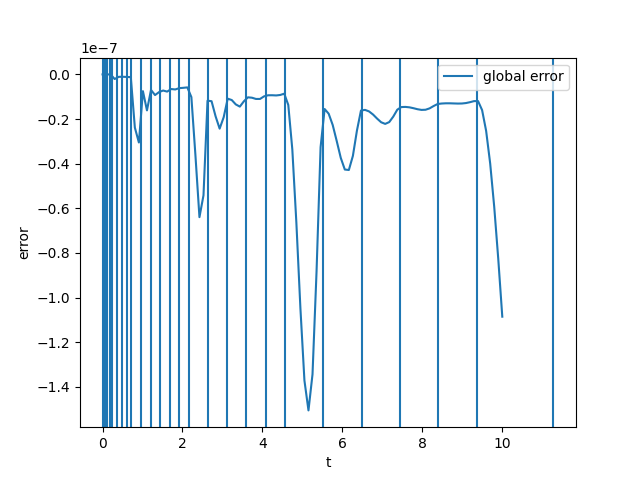
\includegraphics[width=0.7\linewidth]{./figures/static_alpha_rk6_with_hb8_p1_global_error}
\caption{Global Error for RK6 with HB8 using $\alpha$ and $\beta$ = 1 on problem 1 at an absolute tolerance of $10^{-6}$.}
\label{fig:static_alpha_rk6_with_hb8_p1_global_error}
\end{figure}

\begin{figure}[H]
\centering
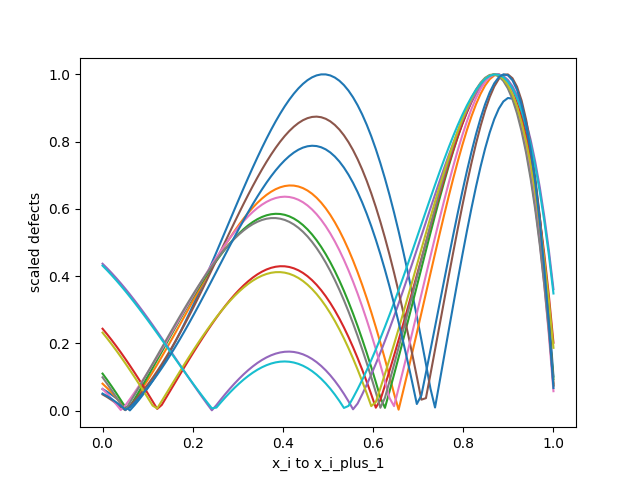
\includegraphics[width=0.7\linewidth]{./figures/static_alpha_rk6_with_hb8_p1_scaled_defects}
\caption{Scaled Defects for RK6 with HB8 using $\alpha$ and $\beta$ = 1 on problem 1 at an absolute tolerance of $10^{-6}$ mapped onto $[0, 1]$.}
\label{fig:static_alpha_rk6_with_hb8_p1_scaled_defects}
\end{figure}

\paragraph{Problem 2 results}
Figures $\ref{fig:static_alpha_rk6_with_hb8_p2_global_defect}$, $\ref{fig:static_alpha_rk6_with_hb8_p2_global_error}$ and $\ref{fig:static_alpha_rk6_with_hb8_p2_scaled_defects}$ shows the results of using RK6 with HB8 and $\alpha = 1$ and $\beta = 1$ on Problem 2. We note that an absolute tolerance of $10^{-6}$ is applied on the maximum defect within the step and this can be shown to occur at $0.8h$ along a step of size, h. See Figure $\ref{fig:static_alpha_rk6_with_hb8_p2_scaled_defects}$, to see the scaled defect reaching a maximum near these points. We note that we are able to successfully control the defect of the continuous numerical solution using this approach, see Figure $\ref{fig:static_alpha_rk6_with_hb8_p2_global_defect}$. 
\begin{figure}[H]
\centering
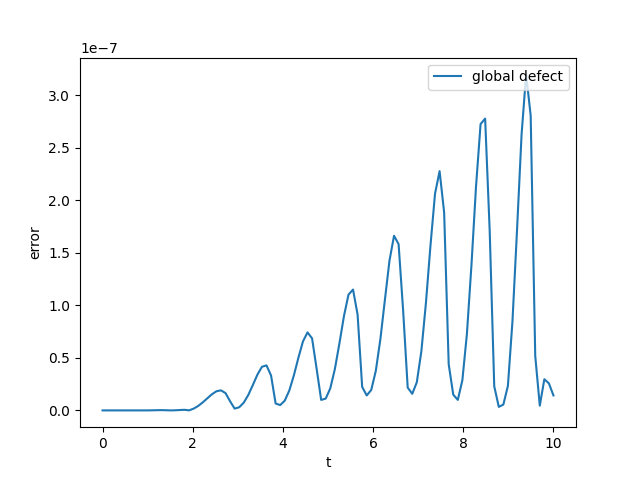
\includegraphics[width=0.7\linewidth]{./figures/static_alpha_rk6_with_hb8_p2_global_defect}
\caption{Defect across the entire domain for RK6 with HB8 using $\alpha$ and $\beta$ = 1 on problem 2 at an absolute tolerance of $10^{-6}$.}
\label{fig:static_alpha_rk6_with_hb8_p2_global_defect}
\end{figure}

\begin{figure}[H]
\centering
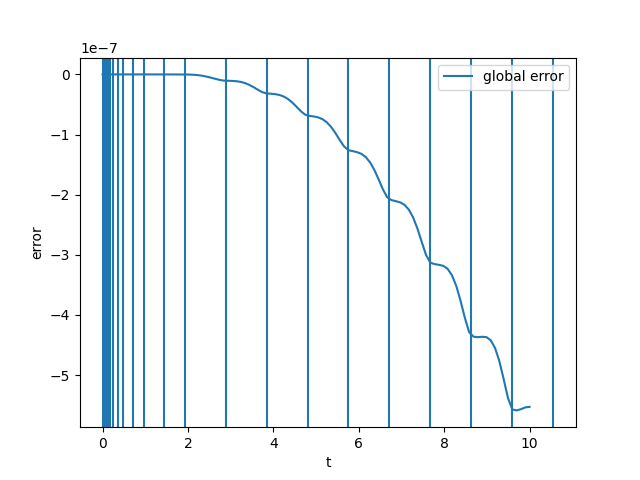
\includegraphics[width=0.7\linewidth]{./figures/static_alpha_rk6_with_hb8_p2_global_error}
\caption{Global Error for RK6 with HB8 using $\alpha$ and $\beta$ = 1 on problem 2 at an absolute tolerance of $10^{-6}$.}
\label{fig:static_alpha_rk6_with_hb8_p2_global_error}
\end{figure}

\begin{figure}[H]
\centering
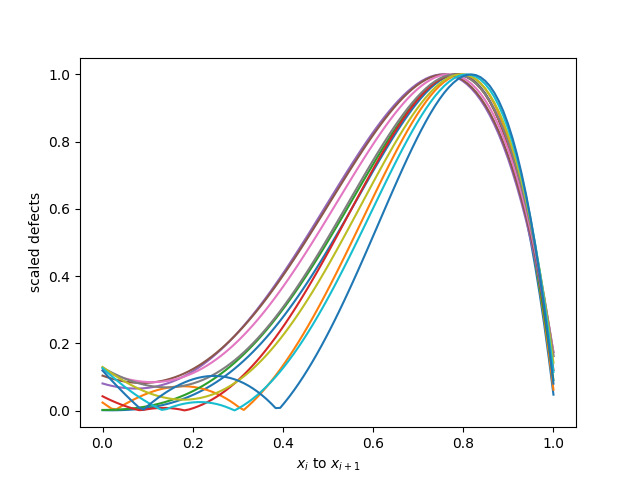
\includegraphics[width=0.7\linewidth]{./figures/static_alpha_rk6_with_hb8_p2_scaled_defects}
\caption{Scaled Defects for RK6 with HB8 using $\alpha$ and $\beta$ = 1 on problem 2 at an absolute tolerance of $10^{-6}$ mapped onto $[0, 1]$.}
\label{fig:static_alpha_rk6_with_hb8_p2_scaled_defects}
\end{figure}

\begin{figure}[H]
\centering
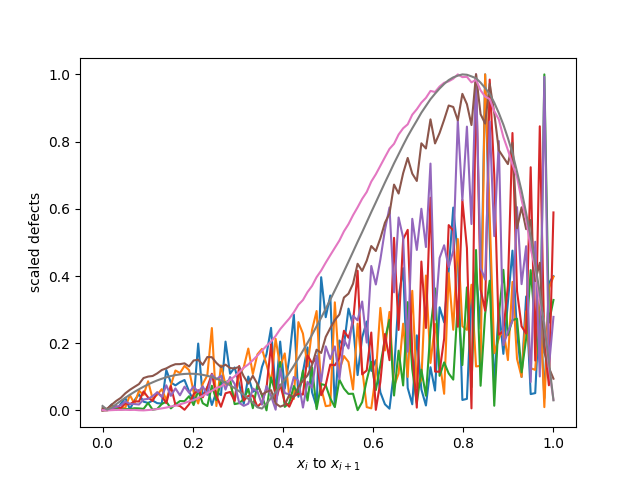
\includegraphics[width=0.7\linewidth]{./figures/static_alpha_rk6_with_hb8_p2_scaled_defects_small_steps}
\caption{Scaled Defects for RK6 with HB8 using $\alpha$ and $\beta$ = 1 on small steps on problem 2 at an absolute tolerance of $10^{-6}$ mapped onto $[0, 1]$. Despite the noise, the maximum defect mostly appears near $0.8h$.}
\label{fig:static_alpha_rk6_with_hb8_p2_scaled_defects_small_steps}
\end{figure}

\paragraph{Problem 3 results}
Figures $\ref{fig:static_alpha_rk6_with_hb8_p3_global_defect}$, $\ref{fig:static_alpha_rk6_with_hb8_p3_global_error}$ and $\ref{fig:static_alpha_rk6_with_hb8_p3_scaled_defects}$ shows the results of using RK6 with HB8 and $\alpha = 1$ and $\beta = 1$ on Problem 3. We note that an absolute tolerance of $10^{-6}$ is applied on the maximum defect within the step and this can be shown to occur at $0.3h$ and $0.8h$ along a step of size, h. See Figure $\ref{fig:static_alpha_rk6_with_hb8_p3_scaled_defects}$, to see the scaled defect reaching a maximum near these points. We note that we are able to successfully control the defect of the continuous numerical solution using this approach, see Figure $\ref{fig:static_alpha_rk6_with_hb8_p3_global_defect}$. 

\begin{figure}[H]
\centering
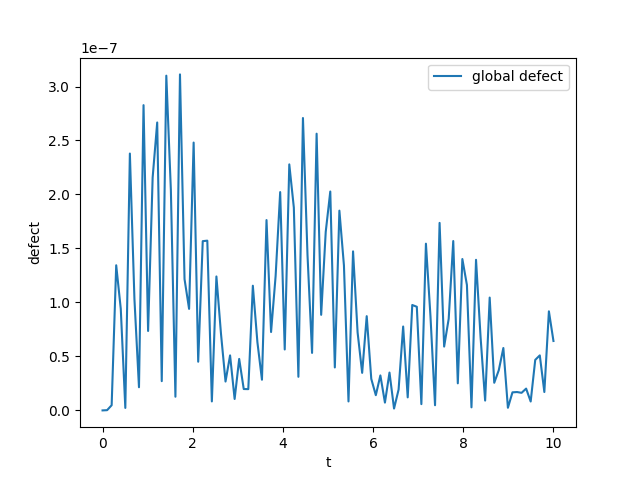
\includegraphics[width=0.7\linewidth]{./figures/static_alpha_rk4_with_hb6_p3_global_defect}
\caption{Defect across the entire domain for RK6 with HB8 using $\alpha$ and $\beta$ = 1 on problem 3 at an absolute tolerance of $10^{-6}$.}
\label{fig:static_alpha_rk6_with_hb8_p3_global_defect}
\end{figure}

\begin{figure}[H]
\centering
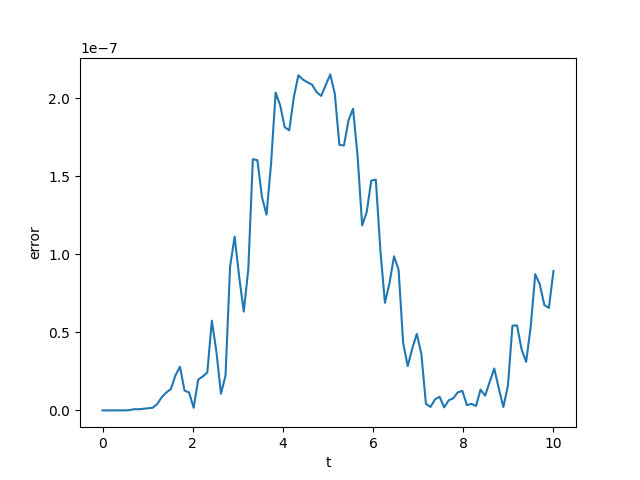
\includegraphics[width=0.7\linewidth]{./figures/static_alpha_rk6_with_hb8_p3_global_error}
\caption{Global Error for RK6 with HB8 using $\alpha$ and $\beta$ = 1 on problem 3 at an absolute tolerance of $10^{-6}$.}
\label{fig:static_alpha_rk6_with_hb8_p3_global_error}
\end{figure}

\begin{figure}[H]
\centering
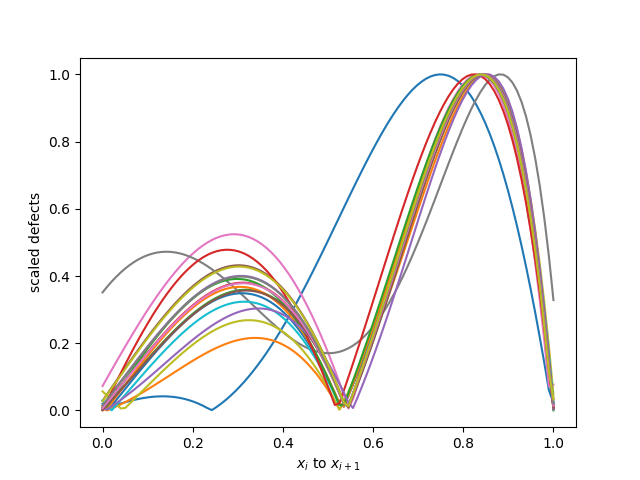
\includegraphics[width=0.7\linewidth]{./figures/static_alpha_rk6_with_hb8_p3_scaled_defects}
\caption{Scaled Defects for RK6 with HB8 using $\alpha$ and $\beta$ = 1 on problem 3 at an absolute tolerance of $10^{-6}$ mapped onto $[0, 1]$.}
\label{fig:static_alpha_rk6_with_hb8_p3_scaled_defects}
\end{figure}

\begin{figure}[H]
\centering
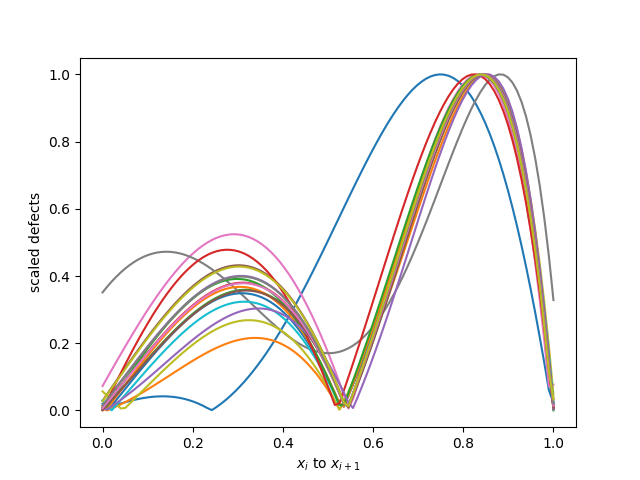
\includegraphics[width=0.7\linewidth]{./figures/static_alpha_rk6_with_hb8_p3_scaled_defects_small_steps}
\caption{Scaled Defects for RK6 with HB8 using $\alpha$ and $\beta$ = 1 on small steps on problem 3 at an absolute tolerance of $10^{-6}$ mapped onto $[0, 1]$. Despite the noise, the maximum defect mostly appears near $0.8h$.}
\label{fig:static_alpha_rk6_with_hb8_p3_scaled_defects_small_steps}
\end{figure}

\begin{table}[h]
\caption {Number of steps taken by RK6 when modified to do defect control with HB8 with $\alpha$ and $\beta$ forcibly at 1 and variable $\alpha$ and $\beta$.} \label{tab:rk6_with_hb8_static_vs_variable}
\begin{center}
\begin{tabular}{ c c c c c } 
Problem & succ. & params=1 succ. steps & nsteps & params=1 nsteps \\ 
1       & 18                      &        23               & 18         & 31\\ 
2       & 14                      &        18               & 17         & 21\\
3       & 24                      &        26               & 26         & 27\\
\end{tabular}
\end{center}
\end{table}	

Table $\ref{tab:rk6_with_hb8_static_vs_variable}$ shows how the solver with $\alpha$ and $\beta$ fixed at 1 and the solver with $\alpha$ and $\beta$ allowed to vary differs in the number of steps that they take. The results are somewhat similar because, as we noted before, $\alpha$ and $\beta$ tends to stay close to 1 and rarely deviates to a value smaller than $\frac{1}{4}$ or larger than 4.

=======================================================
\subsection{rk8 with HB10} For the HB10 case, a simple way to guarantee that the values of $\alpha$ and $\beta$ are 1 is by using the previous interpolants to get the required values at $x_{i - 1}=x_i-2h$ and $x_{i - 2}=x_i-h$. We need to use $2h$ for the $x_{i-1}$ as this step is broken into 2. This way $alpha$ and $beta$ are 1 when we break the step. Suppose that we are at $x_i$ and we took a step of size $h$ to get to the value $x_{i + 1}$ where the function evaluation was $f_{i + 1}$ and the solution was $y_{i + 1}$. We could get the values of the solution and the derivative by using the previous interpolants defined on the range $[0, x_i]$ to get the value at exactly $x_i - 2h$ for the solution, $y_{i - 1}$, and then evaluate $f(t_{i-1}, y_{i-1})$ to get the derivative $f_{i - 1}$.  We can also use the previous interpolants on $[0, x_i]$ to get the values of the solution, $y_{i-2}$ and use it to evaluate $f(t_{i-2}, y_{i-2})$ to get the values of the derivative, $f_{i-2}$, at $x_{i-2} = x_i - 3h$. We could thus create create the new interpolant using the data values defined as such to guarantee that $\alpha$ and $\beta$ equal to 1. We then use the embedded HB8 to get the solution value at $x_{i - \frac{1}{2}}$ and make a function evaluation to get the derivative value. We can then build HB10 on that data. We note that we have built interpolants for both the solution and the derivative that  can interpolate up to $x_i$ for all cases except for the case $x_i = 0$ or for the first few steps. This scheme uses two more function evaluations.

This technique works (see Figures $\ref{fig:static_alpha_rk8_with_hb10_p1_global_defect}$ to $\ref{fig:static_alpha_rk8_with_hb10_p3_scaled_defects}$ to see the defect being controlled) but will require that the step-size is artificially limited on the first few steps so that we can interpolant back $x_i - h$ and/or $x_i - 2h$ and still be in a range where our interpolants are correctly defined. This is not an issue as a CRK scheme could be used for the first few steps.

\paragraph{Problem 1 results}
Figures $\ref{fig:static_alpha_rk8_with_hb10_p1_global_defect}$, $\ref{fig:static_alpha_rk8_with_hb10_p1_global_error}$ and $\ref{fig:static_alpha_rk8_with_hb10_p1_scaled_defects}$ shows the results of using RK8 with HB10 and $\alpha = 1$ and $\beta = 1$ on Problem 1. We note that an absolute tolerance of $10^{-6}$ is applied on the maximum defect within the step and this can be shown to occur at $0.3h$ or $0.8h$ along a step of size, h. See Figure $\ref{fig:static_alpha_rk8_with_hb10_p1_scaled_defects}$, to see the scaled defect reaching a maximum near these points. We note that we are able to successfully control the defect of the continuous numerical solution using this approach, see Figure $\ref{fig:static_alpha_rk8_with_hb10_p1_global_defect}$. 
\begin{figure}[H]
\centering
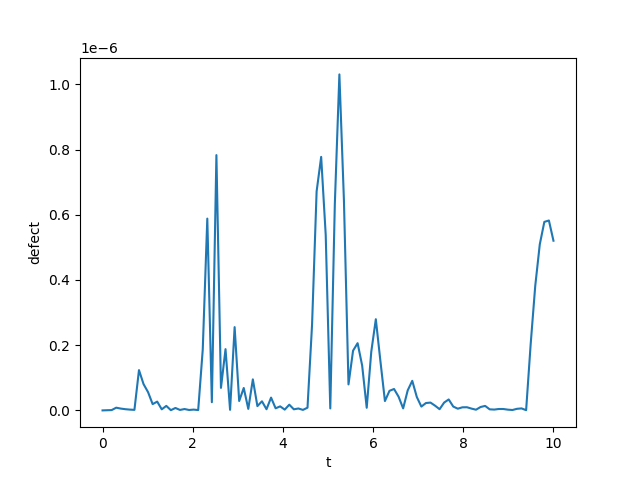
\includegraphics[width=0.7\linewidth]{./figures/static_alpha_rk8_with_hb10_p1_global_defect}
\caption{Defect across the entire domain for RK8 with HB10 using $\alpha$ and $\beta$ = 1 on problem 1 at an absolute tolerance of $10^{-6}$.}
\label{fig:static_alpha_rk8_with_hb10_p1_global_defect}
\end{figure}

\begin{figure}[H]
\centering
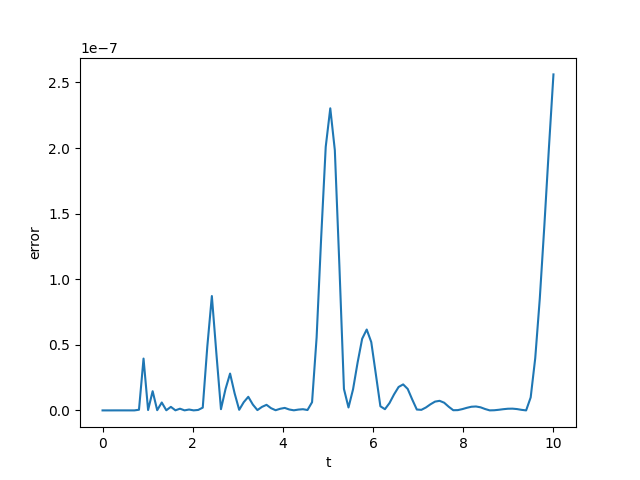
\includegraphics[width=0.7\linewidth]{./figures/static_alpha_rk8_with_hb10_p1_global_error}
\caption{Global Error for RK8 with HB10 using $\alpha$ and $\beta$ = 1 on problem 1 at an absolute tolerance of $10^{-6}$.}
\label{fig:static_alpha_rk8_with_hb10_p1_global_error}
\end{figure}

\begin{figure}[H]
\centering
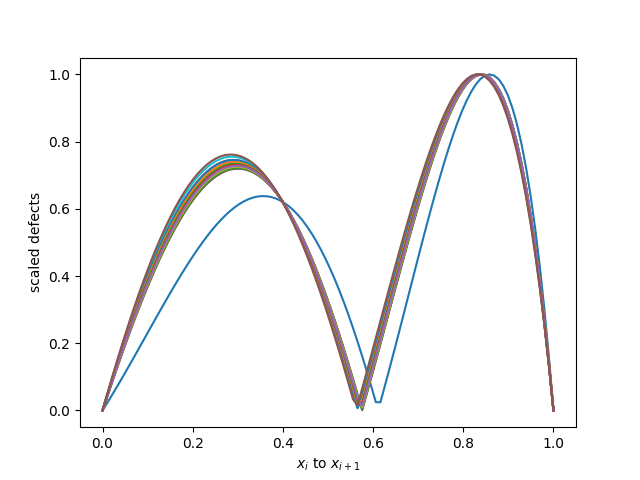
\includegraphics[width=0.7\linewidth]{./figures/static_alpha_rk8_with_hb10_p1_scaled_defects}
\caption{Scaled Defects for RK8 with HB10 using $\alpha$ and $\beta$ = 1 on problem 1 at an absolute tolerance of $10^{-6}$ mapped onto $[0, 1]$.}
\label{fig:static_alpha_rk8_with_hb10_p1_scaled_defects}
\end{figure}

\paragraph{Problem 2 results}
Figures $\ref{fig:static_alpha_rk8_with_hb10_p2_global_defect}$, $\ref{fig:static_alpha_rk8_with_hb10_p2_global_error}$ and $\ref{fig:static_alpha_rk8_with_hb10_p2_scaled_defects}$ shows the results of using RK8 with HB10 and $\alpha = 1$ and $\beta = 1$ on Problem 2. We note that an absolute tolerance of $10^{-6}$ is applied on the maximum defect within the step and this can be shown to occur at $0.8h$ along a step of size, h. See Figure $\ref{fig:static_alpha_rk8_with_hb10_p2_scaled_defects}$, to see the scaled defect reaching a maximum near these points. We note that we are able to successfully control the defect of the continuous numerical solution using this approach, see Figure $\ref{fig:static_alpha_rk8_with_hb10_p2_global_defect}$. 
\begin{figure}[H]
\centering
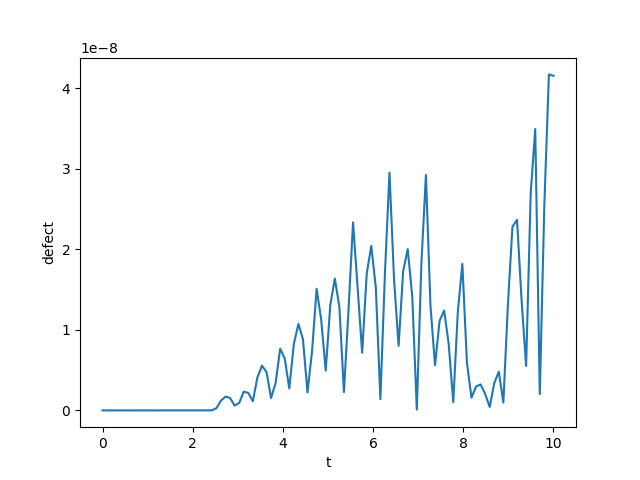
\includegraphics[width=0.7\linewidth]{./figures/static_alpha_rk8_with_hb10_p2_global_defect}
\caption{Defect across the entire domain for RK8 with HB10 using $\alpha$ and $\beta$ = 1 on problem 2 at an absolute tolerance of $10^{-6}$.}
\label{fig:static_alpha_rk8_with_hb10_p2_global_defect}
\end{figure}

\begin{figure}[H]
\centering
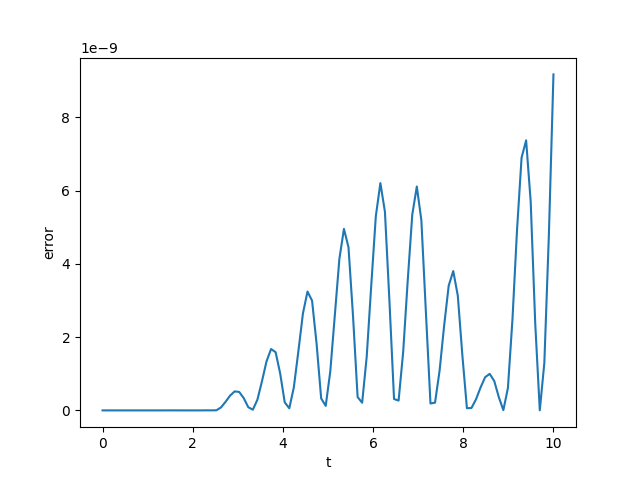
\includegraphics[width=0.7\linewidth]{./figures/static_alpha_rk8_with_hb10_p2_global_error}
\caption{Global Error for RK8 with HB10 using $\alpha$ and $\beta$ = 1 on problem 2 at an absolute tolerance of $10^{-6}$.}
\label{fig:static_alpha_rk8_with_hb10_p2_global_error}
\end{figure}

\begin{figure}[H]
\centering
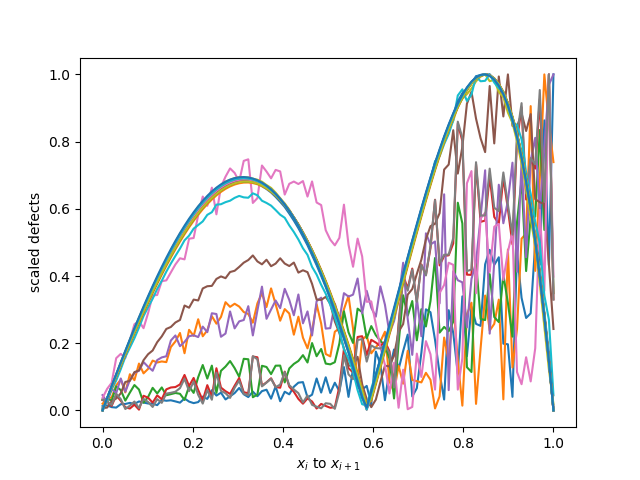
\includegraphics[width=0.7\linewidth]{./figures/static_alpha_rk8_with_hb10_p2_scaled_defects}
\caption{Scaled Defects for RK8 with HB10 using $\alpha$ and $\beta$ = 1 on problem 2 at an absolute tolerance of $10^{-6}$ mapped onto $[0, 1]$.}
\label{fig:static_alpha_rk8_with_hb10_p2_scaled_defects}
\end{figure}

\paragraph{Problem 3 results}
Figures $\ref{fig:static_alpha_rk8_with_hb10_p3_global_defect}$, $\ref{fig:static_alpha_rk8_with_hb10_p3_global_error}$ and $\ref{fig:static_alpha_rk8_with_hb10_p3_scaled_defects}$ shows the results of using RK8 with HB10 and $\alpha = 1$ and $\beta = 1$ on Problem 3. We note that an absolute tolerance of $10^{-6}$ is applied on the maximum defect within the step and this can be shown to occur at $0.3h$ and $0.8h$ along a step of size, h. See Figure $\ref{fig:static_alpha_rk8_with_hb10_p3_scaled_defects}$, to see the scaled defect reaching a maximum near these points. We note that we are able to successfully control the defect of the continuous numerical solution using this approach, see Figure $\ref{fig:static_alpha_rk8_with_hb10_p3_global_defect}$. 

\begin{figure}[H]
\centering
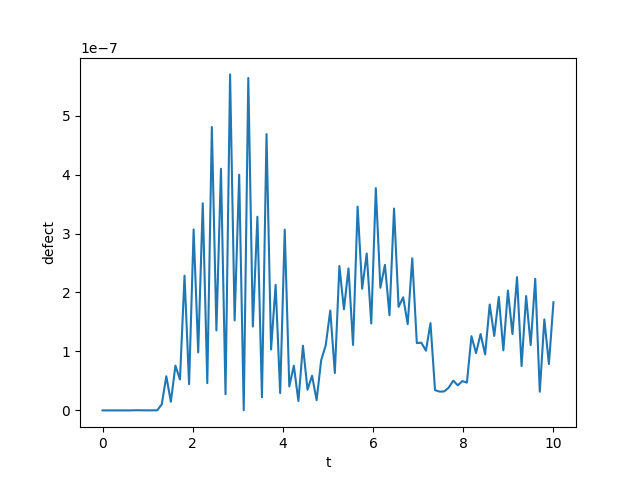
\includegraphics[width=0.7\linewidth]{./figures/static_alpha_rk8_with_hb10_p3_global_defect}
\caption{Defect across the entire domain for RK8 with HB10 using $\alpha$ and $\beta$ = 1 on problem 3 at an absolute tolerance of $10^{-6}$.}
\label{fig:static_alpha_rk8_with_hb10_p3_global_defect}
\end{figure}

\begin{figure}[H]
\centering
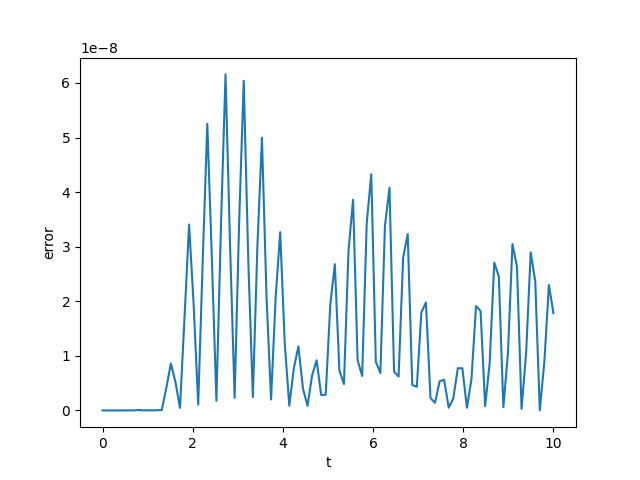
\includegraphics[width=0.7\linewidth]{./figures/static_alpha_rk8_with_hb10_p3_global_error}
\caption{Global Error for RK8 with HB10 using $\alpha$ and $\beta$ = 1 on problem 3 at an absolute tolerance of $10^{-6}$.}
\label{fig:static_alpha_rk8_with_hb10_p3_global_error}
\end{figure}

\begin{figure}[H]
\centering
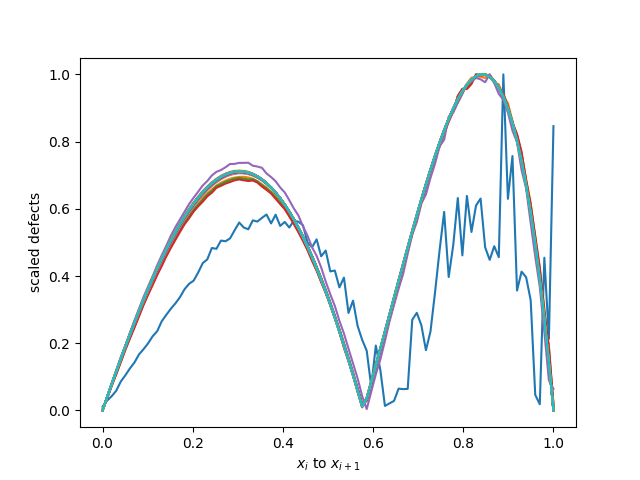
\includegraphics[width=0.7\linewidth]{./figures/static_alpha_rk8_with_hb10_p3_scaled_defects}
\caption{Scaled Defects for RK8 with HB10 using $\alpha$ and $\beta$ = 1 on problem 3 at an absolute tolerance of $10^{-6}$ mapped onto $[0, 1]$.}
\label{fig:static_alpha_rk8_with_hb10_p3_scaled_defects}
\end{figure}


\begin{table}[h]
\caption {Number of steps taken by RK8 when modified to do defect control with HB10 with $\alpha$ and $\beta$ forcibly at 1 and variable $\alpha$ and $\beta$.} \label{tab:rk8_with_hb10_static_vs_variable}
\begin{center}
\begin{tabular}{ c c c c c } 
Problem & succ. & params=1 succ. steps & nsteps & params=1 nsteps \\ 
1       & 14  &        22          & 16   & 35\\ 
2       & 10  &        11          & 13   & 27\\
3       & 20  &        23          & 28   & 32\\
\end{tabular}
\end{center}
\end{table}	

Table $\ref{tab:rk8_with_hb10_static_vs_variable}$ shows that the static parameter version is less efficient. We note that part of this is because of the first steps being wrong but also that the static parameter version is more accurate. This is a problem is the step selection algorithm. A better selection algorithm for such a high order method would drastically reduce the number of failed  steps.